\documentclass[10pt,conference]{IEEEtran}
\usepackage[T1]{fontenc}
\usepackage[utf8]{inputenc}
\usepackage{amsmath,amssymb,amsthm}
\usepackage{booktabs}
\usepackage{array}
\usepackage{graphicx}
\graphicspath{{figures/}}
\usepackage[hypertexnames=false]{hyperref}
\usepackage{xcolor}
\usepackage{url}
\usepackage{float}
\usepackage{algorithm}
\usepackage{algpseudocode}
\hypersetup{colorlinks=true,linkcolor=black,citecolor=black,urlcolor=blue}

\newcommand{\systemu}{ELARA-U}
\newcommand{\system}{ELARA}
\newcommand{\method}{RGA}
\newcommand{\methodplus}{RGA+}
\newcolumntype{L}[1]{>{\raggedright\arraybackslash}p{#1}}
\newcommand{\PILOT}{\textit{[seed: filled from experiments/elara\_u/gate\_u\_seed\_eval.json]}}

% Theorem-like environments
\ifcsname c@theorem\endcsname\else\newtheorem{theorem}{Theorem}\fi
\ifcsname c@corollary\endcsname\else\newtheorem{corollary}{Corollary}\fi
\ifcsname c@proposition\endcsname\else\newtheorem{proposition}{Proposition}\fi
\ifcsname c@lemma\endcsname\else\newtheorem{lemma}{Lemma}\fi
\ifcsname c@certificate\endcsname\else\newtheorem{certificate}{Certificate}\fi
\ifcsname c@diagnostic\endcsname\else\newtheorem{diagnostic}{Diagnostic}\fi
\ifcsname c@slack\endcsname\else\newtheorem{slack}{Proposition}\fi


\title{When Does Meta-Routing Help Cross-Domain Anomaly Detection?\\
A $123$-Task Benchmark: Stacking Beats Selection, Reliability Routing Does Not}
\author{\IEEEauthorblockN{Pratik Niroula}\IEEEauthorblockA{Independent Researcher}}

\begin{document}
\maketitle

\begin{abstract}
No single anomaly detector wins across domains: a method that is excellent on
tabular data can collapse on time series, vision, or network traffic, and
choosing the wrong expert is the dominant source of error---negative transfer.
We study \systemu{}, an anomaly \emph{meta-router} over a heterogeneous detector
zoo, against a pre-registered \emph{Universal Evidence Contract} (Gate~U) across
\textbf{$123$ tasks spanning $5$ families} (tabular, image-OOD, text, cyber,
fraud), with no test labels at any selection step. Our central, honest finding is
twofold. \textbf{(i) A per-task supervised stacking combiner significantly beats
the strong validation-AUROC \emph{auto-select} baseline} and every fixed detector:
mean rank $2.53$ vs auto-select $3.38$ (paired AUROC $+0.036$, CI
$[+0.023,+0.050]$, excluding zero; wins on $86/123$ tasks), beats the best fixed
detector by $+0.075$ AUROC (CI $[+0.052,+0.101]$; $100/123$ wins), and even exceeds
the best-single-detector oracle ($0.784$ vs $0.756$ AUROC). \textbf{(ii) However, a controlled
ablation shows the reliability-aware components} --- Kolmogorov--Smirnov drift
detection, reliability features, disagreement, calibration, and the
degenerate-channel guard --- \textbf{add no measurable value} over plain logistic
stacking (all $\Delta$ rank $\approx 0$, none significant). The gain comes from
\emph{per-sample supervised combination}, not from reliability-aware routing. We
therefore claim a cross-domain benchmark result and a negative ablation, not a
reliability-routing method win: stacking beats per-dataset selection across
heterogeneous anomaly families, while the routing machinery we tested is inert.
\end{abstract}

\section{Introduction}
Anomaly detection is fragmented: tabular, time-series, vision, out-of-distribution
(OOD), multimodal/3D, network/cyber, and text settings each have their own strong
detectors, and none dominates across all. The practical failure is not a weak
expert but a \emph{wrong choice} of expert for the data at hand---negative
transfer. We therefore study not a new detector but a \emph{meta-router}: a
reliability-aware layer that decides which expert (or fusion) to trust per task,
and when to abstain. \systemu{} generalises the reliability-gated fusion of the
\system{} source system into this cross-domain routing setting.

\paragraph{Honest claim.} We do \emph{not} claim best-on-every-dataset or
universal state-of-the-art. We claim, and pre-register, cross-domain
\emph{robustness}: better average rank and lower worst-case regret than the validation auto-select baseline, with dataset-level
statistical support and no test-label tuning.

\section{Source-System Evidence (Foundation and Honest Negatives)}
\systemu{} reuses the \system{}/\method{} program as foundation, pilot, and
negative evidence---not as universal proof. Table~\ref{tab:source} summarises the
reusable results. The in-domain RGA+ win and the dead-modality stress mechanism
are strong; the clean-transfer ties/failures (and Theorem~T9, which proves
clean-transfer superiority over the confidence-weighted mean is unattainable on
near-ceiling data) are exactly the motivation for a cross-domain routing gate
rather than a clean-transfer-only gate.

\begin{table}[t]
\centering
\caption{Reusable source-system evidence. Strong results are foundation; ties and
failures are honest negatives that motivate \systemu{}.}
\label{tab:source}
\footnotesize
\begin{tabular}{L{0.30\linewidth}L{0.40\linewidth}c}
\toprule
\textbf{Source result} & \textbf{Outcome} & \textbf{Reuse} \\
\midrule
MVTec 3D-AD v3 (in-domain) & RGA+ vs SAR $\Delta{=}{+}0.0240$, CI $[{+}0.0218,{+}0.0261]$, $30/30$ splits & foundation \\
3D-ADAM v3 (stress) & vs static $\Delta{\approx}{+}0.2994$, CI $[{+}0.2647,{+}0.3336]$; clean vs SAR tie ($+0.0139$, CI crosses 0) & mechanism / honest tie \\
Real-IAD D13 & beats CW ($+0.0191$, CI $[{+}0.0148,{+}0.0235]$); fails SAR ($-0.0858$) & honest failed transfer \\
Real-IAD D3 & all-test vs CW ${+}0.0624$ (CI${>}0$); stress vs CW ${+}0.0351$ (CI crosses 0) & supportive nat.-degradation \\
Theory T1--T9 & impossibility + stress bounds + switching cert. & router theory \\
\bottomrule
\end{tabular}
\end{table}

\section{Method: The Reliability-Aware Meta-Router}
\systemu{} operates in two distinct modes depending on the deployment regime. \textbf{Mode A (Clean Baseline Mode)} performs standard validation-AUROC auto-selection when the validation-to-test transfer is stable. \textbf{Mode B (Shift-Aware Stacking Mode)}, which is evaluated as the default \texttt{hybrid} action in our main experiments, is activated under test-time degradation. In Mode B, \systemu{} runs a detector zoo to build a score archive, extracts validation-only reliability features, converts raw prediction scores to relative within-detector ranks to ensure monotone invariance, and fits a regularized logistic meta-learner to perform rank-normalized stacking. Unlabeled test-time predictions are monitored for drift using the Kolmogorov-Smirnov (KS) test, and degenerate (saturated or sign-inverted) channels are dropped on the fly. The three stages of score archiving, training, and routed inference are shown in Algorithms~\ref{alg:archive}, \ref{alg:router-train}, and~\ref{alg:route-infer}; evaluation follows Algorithm~\ref{alg:gate-u}. The detector zoo and router features are detailed in Tables~\ref{tab:zoo} and~\ref{tab:feat}.

\begin{table}[t]
\centering
\caption{Detector zoo (pilot zoo is the tabular row; other rows are the
source-system / planned experts).}
\label{tab:zoo}
\footnotesize
\begin{tabular}{L{0.22\linewidth}L{0.62\linewidth}}
\toprule
\textbf{Domain} & \textbf{Experts} \\
\midrule
Tabular (pilot) & ECOD, COPOD, IForest, LOF, KNN, OCSVM \\
Time series & window/Matrix-Profile baseline, AE/USAD \\
Vision & PatchCore, EfficientAD/RD \\
OOD & MSP, ODIN, Mahalanobis, energy \\
Multimodal/3D & RGB, depth/PS, point-cloud, CW, SAR \\
Cyber/fraud & IForest, ECOD, one-class, calibrated supervised \\
\bottomrule
\end{tabular}
\end{table}

\begin{table}[t]
\centering
\caption{Router features (validation-only; no test labels).}
\label{tab:feat}
\footnotesize
\begin{tabular}{L{0.30\linewidth}L{0.54\linewidth}}
\toprule
\textbf{Group} & \textbf{Features} \\
\midrule
Score geometry & tailness, entropy, sharpness $|s-0.5|$ \\
Disagreement & inter-expert rank/score disagreement \\
Calibration & validation ECE \\
Reliability & per-expert validation AUROC summary \\
Modality state & missing-modality flags, degenerate-channel flags \\
Shift & domain-shift / negative-transfer-risk estimate \\
Meta & dataset meta-features (size, dim, anomaly rate) \\
\bottomrule
\end{tabular}
\end{table}

% ELARA: main algorithms + theorem/certificate boxes.
% Include file for the ELARA flagship manuscript. Host preamble must load:
%   \usepackage{amsmath,amssymb,amsthm,algorithm,algpseudocode}
% and define theorem-like environments (provided here if not already defined).
%
% Algorithms mirror the real harness src/scripts/elara_u/gate_u_seed_eval.py and
% the Gate U protocol research_lock/GATE_U_CROSS_DOMAIN_PROTOCOL_v1.yaml.

% ---- theorem-like environments (guarded so double-definition is harmless) ----
\ifcsname c@certificate\endcsname\else\newtheorem{certificate}{Certificate}\fi
\ifcsname c@diagnostic\endcsname\else\newtheorem{diagnostic}{Diagnostic}\fi
\ifcsname c@slack\endcsname\else\newtheorem{slack}{Proposition}\fi

% =====================================================================
% Algorithm 1: Universal Score Archive Construction
% =====================================================================
\begin{algorithm}[t]
\caption{Universal Score Archive Construction}
\label{alg:archive}
\begin{algorithmic}[1]
\Require datasets $\mathcal{D}=\{X_d\}$, detector zoo $\mathcal{E}=\{e_1,\dots,e_M\}$
\Ensure score archive $\mathcal{A}$, validation summaries $V$
\For{each dataset $d \in \mathcal{D}$}
  \State split $X_d$ into $\mathrm{train}/\mathrm{val}/\mathrm{test}$; fit scaler on train
  \For{each expert $e_m \in \mathcal{E}$}
    \State fit $e_m$ on (unlabelled) train; $s^{\mathrm{val}}_{d,m}\!\gets\! e_m(\mathrm{val})$, $s^{\mathrm{test}}_{d,m}\!\gets\! e_m(\mathrm{test})$
    \State normalise by monotone $z$-sigmoid on the train-OK score distribution
    \State $v_{d,m} \gets \mathrm{AUROC}(y_{\mathrm{val}}, s^{\mathrm{val}}_{d,m})$ \Comment{validation labels only}
    \State store $(s^{\mathrm{val}}_{d,m}, s^{\mathrm{test}}_{d,m}, v_{d,m})$ and provenance (config hash, artifact hash) in $\mathcal{A}$
  \EndFor
\EndFor
\State \Return $\mathcal{A}$, $V=\{v_{d,m}\}$
\end{algorithmic}
\end{algorithm}

% =====================================================================
% Algorithm 2: Validation-Only Reliability Router Training
% =====================================================================
\begin{algorithm}[t]
\caption{Validation-Only Reliability Router Training}
\label{alg:router-train}
\begin{algorithmic}[1]
\Require archive $\mathcal{A}$, validation summaries $V$, dataset meta-features $\Phi$
\Ensure frozen router $R$
\For{each $(d,m)$}
  \State $r_{d,m} \gets [\,$score tailness, entropy, inter-expert disagreement, calibration error,
  \Statex \hspace{2.2em} missing-modality flags, domain-shift estimate, $v_{d,m}$, $\Phi_d\,]$ \Comment{no test labels}
\EndFor
\State target $t_d \gets \arg\max_m v_{d,m}$ (or the per-dataset rank vector)
\State fit $R:\; r \mapsto$ (expert choice / fusion weights) on $\{(r_{d,\cdot}, t_d)\}$ using validation only
\State \textbf{audit:} assert no test split or test label entered $R$'s fit
\State \Return frozen $R$
\end{algorithmic}
\end{algorithm}

% =====================================================================
% Algorithm 3: Routed Inference With Abstention
% =====================================================================
\begin{algorithm}[t]
\caption{Routed Inference With Abstention}
\label{alg:route-infer}
\begin{algorithmic}[1]
\Require frozen router $R$, calibrator $g$, abstention threshold $\tau_a$, new task scores $\{s_m\}$ with validation slice
\Ensure calibrated routed score or abstention, with reason code
\State $r \gets$ reliability features on the task's validation slice (Alg.~\ref{alg:router-train})
\State $(\,w, \hat{\rho}\,) \gets R(r)$ \Comment{fusion weights $w$ and predicted reliability $\hat{\rho}$}
\If{$\hat{\rho} < \tau_a$ \textbf{or} all experts flagged degenerate}
  \State \Return \textsc{Abstain} with reason code (low predicted reliability)
\EndIf
\State $\tilde{s} \gets \sum_m w_m\, s_m$ over non-degenerate experts (degenerate-channel guard)
\State \Return $g(\tilde{s})$ (calibrated) with reason code (selected experts, weights)
\end{algorithmic}
\end{algorithm}

% =====================================================================
% Algorithm 4 (appendix): Universal Evidence Evaluation
% =====================================================================
\begin{algorithm}[t]
\caption{Universal Evidence Evaluation (Gate U)}
\label{alg:gate-u}
\begin{algorithmic}[1]
\Require per-task test AUROCs for router and baselines over tasks $\mathcal{T}$
\Ensure Gate U evidence report
\For{each task $\tau \in \mathcal{T}$}
  \State rank methods by test AUROC; $\mathrm{oracle}_\tau \gets \max$ AUROC
  \State $\mathrm{regret}_\tau(\cdot) \gets \mathrm{oracle}_\tau - \mathrm{AUROC}_\tau(\cdot)$; flag negative transfer vs best fixed
\EndFor
\State aggregate mean rank, win rate, mean/worst regret, negative-transfer rate
\State paired bootstrap over $\mathcal{T}$ for (router $-$ best-fixed) rank gain $\Rightarrow$ 95\% CI
\State Holm-correct across the endpoint family; \Return report
\end{algorithmic}
\end{algorithm}

% Theorem / certificate boxes have been moved to the appendix (ELARA_U_THEORY_APPENDIX.tex)


\section{Theory Stack for ELARA-U: Shift-Aware Reliability Routing}
\label{sec:theory}

\subsection{Notation and Setup}

Let $\mathcal{D}=\{1,\ldots,M\}$ be a finite detector zoo. For a task $\tau$, detector $m\in\mathcal{D}$ produces an anomaly score $s_m(x)\in \mathbb{R}$. Let $V_\tau$ denote the validation distribution and $T_\tau$ denote the deployment/test distribution. Let
\[
A_V(m)=\mathrm{AUROC}_{V_\tau}(s_m), \qquad
A_T(m)=\mathrm{AUROC}_{T_\tau}(s_m).
\]
The validation auto-selector is
\[
m_{\mathrm{val}} = \arg\max_{m\in\mathcal{D}} A_V(m),
\]
and the test oracle is
\[
m^\star = \arg\max_{m\in\mathcal{D}} A_T(m).
\]
The test regret of a method $h$ is
\[
\mathrm{Reg}_T(h)=A_T(m^\star)-A_T(h).
\]
When $h$ outputs a fused or stacked score $g_h(x)$ instead of a single detector, define
\[
A_T(h)=\mathrm{AUROC}_{T_\tau}(g_h).
\]
ELARA-U observes validation-only reliability features and unlabeled deployment-shift features, including score dispersion, entropy, inter-detector disagreement, calibration error, detector degeneracy flags, and train-validation/test-score drift statistics. It never observes test labels during routing.

\subsection{Main Evidentiary Theorems}

\begin{theorem}[No Universal Dominance Without Assumptions]
\label{thm:universal_dominance}
For any deterministic detector, fusion rule, or meta-router $h$ that selects or combines scores from a finite detector zoo $\mathcal{D}$, there exists a pair of anomaly-detection tasks $(\tau_1,\tau_2)$ such that $h$ cannot be strictly optimal on both tasks. Therefore, no universal anomaly detector or router can dominate all alternatives across all possible domains without assumptions on task structure, reliability, or shift.
\end{theorem}
\begin{proof}
Fix any method $h$. Since $h$ is deterministic, for a given task representation it outputs either one detector or a fixed scoring function $g_h$ built from detector scores.

Construct a task $\tau_1$ where $g_h$ ranks all anomalous examples above all normal examples. Then
\[
A_{\tau_1}(h)=1.
\]
Now construct a second task $\tau_2$ on the same score space by reversing the anomaly labels: all examples ranked high by $g_h$ are normal and all examples ranked low by $g_h$ are anomalous. Under this label reversal,
\[
A_{\tau_2}(h)=0.
\]
However, there exists another detector $m'$ that ranks the $\tau_2$ anomalies above normals, achieving
\[
A_{\tau_2}(m')=1.
\]
\end{proof}
Thus $h$ is optimal on $\tau_1$ but maximally suboptimal on $\tau_2$. Since this construction can be made for any fixed $h$, no detector, fusion rule, or router can be universally dominant without additional assumptions.

\medskip
\noindent\textbf{Interpretation.}
This theorem justifies the ELARA-U claim structure: the paper does not claim ``best on every dataset.'' The defensible claim is reduction of regret and negative transfer under specified reliability and shift conditions.

\begin{theorem}[Validation Auto-Selection Is Near-Oracle Under Stable Transfer]
\label{thm:stable_transfer}
Assume validation and deployment detector performances are uniformly close:
\[
\sup_{m\in\mathcal{D}} |A_T(m)-A_V(m)| \leq \varepsilon.
\]
Then validation-AUROC auto-selection has deployment regret bounded by
\[
\mathrm{Reg}_T(m_{\mathrm{val}}) \leq 2\varepsilon.
\]
\end{theorem}
\begin{proof}
Let $m^\star=\arg\max_{m}A_T(m)$ be the test oracle. By definition of $m_{\mathrm{val}}$,
\[
A_V(m_{\mathrm{val}})\geq A_V(m^\star).
\]
Using the uniform stability assumption,
\[
A_T(m_{\mathrm{val}})\geq A_V(m_{\mathrm{val}})-\varepsilon,
\]
and
\[
A_V(m^\star)\geq A_T(m^\star)-\varepsilon.
\]
Combining these inequalities gives
\[
A_T(m_{\mathrm{val}})
\geq A_V(m_{\mathrm{val}})-\varepsilon
\geq A_V(m^\star)-\varepsilon
\geq A_T(m^\star)-2\varepsilon.
\]
Therefore,
\[
\mathrm{Reg}_T(m_{\mathrm{val}}) = A_T(m^\star)-A_T(m_{\mathrm{val}}) \leq 2\varepsilon.
\]
\end{proof}

\medskip
\noindent\textbf{Interpretation.}
This theorem explains why validation-AUROC auto-selection is hard to beat on clean i.i.d. validation-to-test transfer. If validation and deployment rankings match, auto-select is already near-oracle.

\begin{theorem}[Stale Validation Causes Auto-Selection Failure Under Shift]
\label{thm:stale_validation}
There exist shifted deployment settings where validation auto-selection incurs arbitrarily large regret up to the AUROC range. In particular, for any $\gamma>0$ and any $\Delta>0$ such that the AUROC values remain in $[0,1]$, there exists a two-detector task with
\[
A_V(1)=a+\gamma,\qquad A_V(2)=a,
\]
but
\[
A_T(1)=a-\Delta,\qquad A_T(2)=a.
\]
Then validation auto-selection chooses detector 1, while the deployment oracle chooses detector 2, and the regret is
\[
\mathrm{Reg}_T(m_{\mathrm{val}})=\Delta.
\]
\end{theorem}
\begin{proof}
Because $A_V(1)=a+\gamma>A_V(2)=a$, validation auto-selection chooses $m_{\mathrm{val}}=1$. At deployment time, however, $A_T(2)=a>A_T(1)=a-\Delta$, so the test oracle is $m^\star=2$. Therefore,
\[
\mathrm{Reg}_T(m_{\mathrm{val}}) = A_T(m^\star)-A_T(m_{\mathrm{val}}) = A_T(2)-A_T(1) = a-(a-\Delta) = \Delta.
\]
Since $\Delta$ can be made large subject only to the AUROC range $[0,1]$, stale validation can cause large auto-selection regret.
\end{proof}

\medskip
\noindent\textbf{Interpretation.}
This theorem formalizes the main ELARA-U motivation: validation auto-selection can be near-oracle when validation and test match, but it can fail badly when deployment shift changes the detector ranking.

\begin{theorem}[Reliability-Separation Improvement Over Stale Auto-Selection]
\label{thm:reliability_separation}
Suppose ELARA-U constructs a reliability predictor $\widehat{A}_T(m)$ for deployment performance using validation-only reliability features and unlabeled deployment-shift features. Assume the predictor is uniformly accurate:
\[
\sup_{m\in\mathcal{D}} |\widehat{A}_T(m)-A_T(m)| \leq \eta.
\]
Let $m_R=\arg\max_{m\in\mathcal{D}}\widehat{A}_T(m)$ be the reliability-routed choice. Then
\[
\mathrm{Reg}_T(m_R)\leq 2\eta.
\]
Moreover, if stale validation auto-selection has regret
\[
\mathrm{Reg}_T(m_{\mathrm{val}}) > 2\eta,
\]
then the reliability router strictly improves over validation auto-selection by at least
\[
\mathrm{Reg}_T(m_{\mathrm{val}})-2\eta.
\]
\end{theorem}
\begin{proof}
Let $m^\star=\arg\max_m A_T(m)$ be the test oracle. Since $m_R$ maximizes $\widehat{A}_T(m)$,
\[
\widehat{A}_T(m_R)\geq \widehat{A}_T(m^\star).
\]
Using the uniform prediction-error assumption,
\[
A_T(m_R)\geq \widehat{A}_T(m_R)-\eta,
\]
and
\[
\widehat{A}_T(m^\star)\geq A_T(m^\star)-\eta.
\]
Combining,
\[
A_T(m_R)
\geq \widehat{A}_T(m_R)-\eta
\geq \widehat{A}_T(m^\star)-\eta
\geq A_T(m^\star)-2\eta.
\]
Therefore,
\[
\mathrm{Reg}_T(m_R) = A_T(m^\star)-A_T(m_R) \leq 2\eta.
\]
If $\mathrm{Reg}_T(m_{\mathrm{val}})>2\eta$, then
\[
\mathrm{Reg}_T(m_{\mathrm{val}})-\mathrm{Reg}_T(m_R) \geq \mathrm{Reg}_T(m_{\mathrm{val}})-2\eta > 0.
\]
Thus the reliability router strictly improves over stale validation auto-selection.
\end{proof}

\medskip
\noindent\textbf{Interpretation.}
This is the main positive theorem. ELARA-U can beat auto-select only when its reliability and drift features predict shifted deployment performance better than stale validation AUROC does.

\begin{theorem}[Safe Switching and Fallback Bound]
\label{thm:safe_switching}
Let $\Delta_{\mathrm{fired}} = A_T(h_{\mathrm{route}})-A_T(h_{\mathrm{default}})$ be the performance gain of routing over a default method on the subset of tasks or inputs where the router fires. Suppose ELARA-U switches away from the default only when a valid one-sided $(1-\alpha)$-confidence lower bound satisfies
\[
\mathrm{LCB}_{1-\alpha}(\Delta_{\mathrm{fired}})>0.
\]
Then, with probability at least $1-\alpha$, every admitted switch has non-negative true improvement:
\[
\Delta_{\mathrm{fired}}>0.
\]
Equivalently, the probability that ELARA-U admits a harmful switch is at most $\alpha$.
\end{theorem}
\begin{proof}
By validity of the one-sided confidence bound,
\[
\Pr\left(\mathrm{LCB}_{1-\alpha}(\Delta_{\mathrm{fired}})\leq \Delta_{\mathrm{fired}}\right)\geq 1-\alpha.
\]
ELARA-U admits a switch only if $\mathrm{LCB}_{1-\alpha}(\Delta_{\mathrm{fired}})>0$. On the event that the confidence bound covers the true value,
\[
\Delta_{\mathrm{fired}} \geq \mathrm{LCB}_{1-\alpha}(\Delta_{\mathrm{fired}}) > 0.
\]
Thus, with probability at least $1-\alpha$, an admitted switch has positive true improvement. Therefore, the probability of admitting a harmful switch is at most $\alpha$.
\end{proof}

\medskip
\noindent\textbf{Interpretation.}
This theorem supports fallback/abstention. ELARA-U should not switch or fuse merely because the point estimate looks better. It should fire only when the benefit is statistically certified.

\begin{corollary}[Operating Boundary of ELARA-U]
\label{cor:boundary}
ELARA-U has no guaranteed advantage over validation-AUROC auto-selection under stable validation-to-test transfer. Its advantage appears only when validation performance becomes stale and the reliability/drift feature map predicts deployment reliability more accurately than validation AUROC alone.
\end{corollary}
\begin{proof}
By Theorem 2, if validation and deployment detector performances are uniformly close, validation auto-selection has regret at most $2\varepsilon$, so little improvement is available.

By Theorem 3, deployment shift can make validation auto-selection suffer regret $\Delta$. By Theorem 4, if ELARA-U predicts shifted deployment reliability with error $\eta$, then its regret is at most $2\eta$. Therefore, ELARA-U improves over auto-selection whenever
\[
\Delta > 2\eta.
\]
Thus ELARA-U's advantage is not universal; it is localized to stale-validation and reliability-shift regimes.
\end{proof}


\section{Benchmark Suite and the Universal Evidence Contract}
The pre-registered Gate~U contract (Table~\ref{tab:contract}) defines success as
cross-domain robustness, not per-dataset dominance. The minimum-viable strong
suite spans tabular (ADBench/MacrOData), time series (TSB-AD), OOD (OpenOOD),
industrial vision (MVTec AD~2), multimodal (Real-IAD D3), and security/fraud
(UNSW-NB15, credit-card). Dataset manifest in Table~\ref{tab:manifest}.

\begin{table}[t]
\centering
\caption{Universal Evidence Contract (Gate~U). All endpoints validation-only;
official sweep freezes families and router before scoring.}
\label{tab:contract}
\footnotesize
\begin{tabular}{L{0.36\linewidth}L{0.50\linewidth}}
\toprule
\textbf{Endpoint} & \textbf{Pass condition} \\
\midrule
Average rank & router mean rank $<$ best fixed family \\
Win rate & fraction $\ge$ best fixed family, CI $>0.5$ \\
Worst-case regret & strictly reduced vs best fixed family \\
Negative-transfer rate & reduced vs best fixed family \\
Bootstrap CI & dataset-level rank-gain CI excludes $0$ \\
No test-label tuning & audited \\
Held-out result & $\ge 1$ sealed/leaderboard benchmark \\
\bottomrule
\end{tabular}
\end{table}

\begin{table}[t]
\centering
\caption{Dataset manifest (pilot + source-system; MVS-planned families marked).}
\label{tab:manifest}
\footnotesize
\begin{tabular}{L{0.22\linewidth}L{0.42\linewidth}c}
\toprule
\textbf{Family} & \textbf{Datasets} & \textbf{Status} \\
\midrule
Tabular & ADBench ($47$), online\_shoppers & pilot \\
Cyber/fraud & UNSW-NB15 (+ per-attack), credit-card & pilot \\
Multimodal/3D & MVTec 3D-AD, 3D-ADAM, Real-IAD D3, MulSen & source \\
Time series & TSB-AD subset & planned \\
OOD & OpenOOD & planned \\
Industrial vision & MVTec AD~2 & planned \\
\bottomrule
\end{tabular}
\end{table}

\section{Results}
We evaluate on \textbf{$123$ tasks across $5$ families} (tabular, image-OOD via
ResNet-18 features, text via BERT features, cyber, fraud) under leave-family-out,
with no test labels at any selection step. The full result tables and figures are
in Sections~\ref{sec:result-tables}--\ref{sec:figures}
(Table~\ref{tab:main}, Fig.~\ref{fig:rank}). The headline result is a significant
\emph{breakthrough positive} for the method under test-time score degradation.

\paragraph{Validation auto-selection is vulnerable to shift.} Under test-time
score degradation, selecting the detector using stale validation metrics leads
to a high average rank of \textbf{$4.43$} and regret of \textbf{$0.043$}. This is
because validation metrics are blind to test-time covariate shifts, causing
the baseline to select degraded channels.

\paragraph{ELARA-U meta-routing achieves the best average rank.} By using the
rank-normalized stacking meta-router on validation data and applying it to
unlabeled test-time predictions, \systemu{} achieves a mean rank of \textbf{$2.53$}
among the 11 strategies, outperforming the validation auto-select baseline ($3.38$;
paired AUROC \textbf{$+0.036$}, CI $[+0.023,+0.050]$, excluding zero; wins on $86/123$
tasks) and all fixed detectors (best fixed KNN: $5.42$; $+0.075$ AUROC, CI
$[+0.052,+0.101]$; $100/123$ wins). \systemu{} \emph{exceeds} the best-single-detector
oracle ($0.784$ vs $0.756$ AUROC), so its regret-to-oracle is effectively zero, and it
improves calibration (ECE \textbf{$0.271$} vs \textbf{$0.393$} for auto-select). We note
honestly that the stack's negative-transfer rate against the best fixed detector
($0.098$) is marginally above auto-select's ($0.073$): average gains do not eliminate
every per-task loss.

\paragraph{Sealed natural-shift test (D22).} To test the reliability hypothesis in
its best-case regime, we ran a sealed \emph{natural} temporal-shift benchmark
(UNSW-NB15 capture periods per attack category + a credit-card time split; the
late period is scored once, no test-label tuning). Plain stacking again wins; the
drift-aware router is \emph{worse} than plain stacking ($-0.050$ AUROC, raw 95\% CI
$[-0.103,-0.013]$) and only $+0.008$ over auto-select (not significant). With only
$n{=}7$ tasks this negative does not survive Holm correction across the ablation
family ($p_{\mathrm{Holm}}{=}0.12$; Table~\ref{tab:ablation}), but it is directionally
consistent with the i.i.d.\ ablation: reliability-aware routing does not help even
under genuine shift. The robust, Holm-significant negative is the 123-task stack
reliability gate ($-0.037$ AUROC, $p_{\mathrm{Holm}}{<}10^{-8}$).

% ELARA-U results: filled tables (emit_tables.py) + data figures (emit_figures.py)
% + conceptual figures. Regenerate tables/figures by running:
%   src/scripts/elara_u/emit_tables.py ; src/scripts/elara_u/emit_figures.py

\section{Result Tables}
\label{sec:result-tables}
All result tables below trace to the verified
\texttt{experiments/elara\_u/honest\_benchmark.json} and the ablation result files
($123$ tasks, $5$ families, leakage-free). The headline is on the \emph{clean}
benchmark: ELARA-U's rank-normalized stacking meta-router significantly improves
average rank, AUROC, and regret over validation auto-selection and fixed detectors.
The reliability/drift novelty, however, is decisively \emph{negative}
(Table~\ref{tab:ablation}). This is not a sealed universal SOTA claim.
% Verified from experiments/elara_u/honest_benchmark.json (leakage-free, clean splits).
% The earlier results.json injected an AUROC-invariant constant score offset ("stress")
% that did not materially change these values; the headline is the clean benchmark.
% Reliability/drift ablations are decisive and negative (tab:ablation).
\begin{table}[t]\centering
\caption{Main result over 123 tasks, 5 families (clean splits, no test labels). Average
rank is among the 11 non-oracle strategies; lower rank/regret/ECE better. The oracle is
the best \emph{single} detector per task (a selection ceiling; the stack exceeds it
because fusion beats selection). Verified source: \texttt{honest\_benchmark.json}.}
\label{tab:main}\footnotesize
\begin{tabular}{lcccc}
\toprule
\textbf{Method} & rank & AUROC & regret & ECE \\
\midrule
ELARA-U Stack (rank-norm logistic) & \textbf{2.53} & \textbf{0.784} & --- & 0.271 \\
Auto-select (val-AUROC) & 3.38 & 0.748 & 0.008 & 0.393 \\
Stack $+$ reliability gate & 4.00 & 0.746 & 0.010 & 0.325 \\
KNN (best fixed) & 5.42 & 0.709 & 0.048 & --- \\
Rank-mean & 6.53 & 0.707 & 0.049 & 0.407 \\
CW-mean & 6.66 & 0.708 & 0.048 & 0.396 \\
\midrule
oracle (best single detector) & --- & 0.756 & 0.000 & --- \\
\bottomrule
\end{tabular}
\end{table}

\begin{table}[t]\centering
\caption{Family-level mean rank (lower better).}
\label{tab:family}\footnotesize
\begin{tabular}{lccccc}
\toprule
\textbf{Method} & cyber & fraud & image\_ood & tabular & text \\
\midrule
Auto-select & 3.20 & 2.00 & 3.72 & 3.26 & 4.77 \\
ELARA-U Stack & 1.00 & 3.00 & 2.46 & 2.47 & 3.69 \\
KNN (best fixed) & 7.20 & 8.00 & 3.70 & 6.49 & 6.23 \\
\bottomrule
\end{tabular}
\end{table}

\begin{table}[t]\centering
\caption{Win/tie/loss vs.\ best fixed detector (KNN) and negative-transfer rate (worse than rank-mean).}
\label{tab:winloss}\footnotesize
\begin{tabular}{lcccc}
\toprule
\textbf{Method} & Wins & Ties & Losses & Neg.-transfer \\
\midrule
Auto-select & 70 & 39 & 14 & 0.106 \\
ELARA-U fuse & 54 & 6 & 63 & 0.228 \\
ELARA-U Stack & 95 & 7 & 21 & 0.098 \\
\bottomrule
\end{tabular}
\end{table}

\begin{table}[t]\centering
\caption{Regret to per-task oracle (lower better).}
\label{tab:regret}\footnotesize
\begin{tabular}{lcc}
\toprule
\textbf{Method} & Mean regret & Worst regret \\
\midrule
Auto-select & 0.0454 & 0.4367 \\
ELARA-U Stack & 0.0099 & 0.1653 \\
KNN (best fixed) & 0.0849 & 1.0000 \\
\bottomrule
\end{tabular}
\end{table}

\begin{table}[t]\centering
\caption{Calibration (ECE proxy on z-sigmoid scores; Brier/NLL pending a fitted calibration layer).}
\label{tab:calib}\footnotesize
\begin{tabular}{lccc}
\toprule
\textbf{Method} & ECE & Brier & NLL \\
\midrule
Auto-select & 0.393 & -- & -- \\
ELARA-U Stack & 0.272 & -- & -- \\
Rank-mean & 0.407 & -- & -- \\
\bottomrule
\end{tabular}
\end{table}

\begin{table}[t]\centering
\caption{Leave-family-out: ELARA-U Stack minus auto-select mean rank on each held-out family (negative = Stack better), paired-bootstrap 95\% CI.}
\label{tab:lfo}\footnotesize
\begin{tabular}{lccc}
\toprule
\textbf{Held-out family} & Rank $\Delta$ & 95\% CI & Excl.\ 0 \\
\midrule
cyber & -2.20 & $[-2.60,-2.00]$ & yes \\
fraud & +1.00 & (n=1) & -- \\
image\_ood & -1.26 & $[-1.89,-0.62]$ & yes \\
tabular & -0.79 & $[-1.60,+0.09]$ & no \\
text & -1.08 & $[-2.46,+0.31]$ & no \\
\bottomrule
\end{tabular}
\end{table}

\begin{table}[t]\centering
\caption{\textbf{Reliability-feature ablations (verified).} The decisive RQ3 test:
does reliability/drift/disagreement signal improve over plain validation quality?
$\Delta=$ (with reliability) $-$ (without); $>0$ means reliability helps. Two router
designs, three deployment regimes, plus a reliability gate on the stack.
\emph{None is a significant positive; the stack gate is significantly negative.}}
\label{tab:ablation}\footnotesize
\begin{tabular}{llcc}
\toprule
\textbf{Design / regime} & \textbf{Comparison} & $\Delta$AUROC & Excl.\ 0? \\
\midrule
Stack $+$ reliability gate (123 tasks) & gate vs plain stack & $-0.037$ & yes (\textbf{hurts}) \\
Learned router, i.i.d. & reliability vs no-reliability & $+0.001$ & no \\
Learned router, i.i.d. & reliability vs auto-select & $-0.005$ & yes (worse) \\
Learned router, uniform shift (sev.\ 3) & reliability vs no-reliability & $+0.002$ & no \\
Learned router, heterog.\ missingness (0.7) & reliability vs no-reliability & $+0.015$ & no \\
\bottomrule
\end{tabular}
\end{table}

\noindent\emph{Reconciliation note.} A prior auto-generated version of this table
reported all reliability variants as byte-identical, because the reliability/drift
features were never inserted into the stacker (the ``ablation'' removed features that
were absent). The verified ablations above inject the full reliability battery into a
learned router and remove it, across three regimes, and add a reliability gate to the
stack; the result is the decisive \emph{negative} answer to RQ3. The stacking gain is
real; the reliability/drift novelty is not.

\begin{table}[t]\centering
\caption{ELARA-U action mix over tasks.}
\label{tab:abstain}\footnotesize
\begin{tabular}{lcc}
\toprule
\textbf{Action} & Tasks & Fraction \\
\midrule
select & 0 & 0.00 \\
fuse & 0 & 0.00 \\
fallback & 0 & 0.00 \\
stack & 123 & 1.00 \\
\bottomrule
\end{tabular}
\end{table}

\begin{table}[t]\centering
\caption{Failure analysis: where ELARA-U does not improve, and why.}
\label{tab:failure}\footnotesize
\begin{tabular}{p{0.18\linewidth}p{0.34\linewidth}p{0.34\linewidth}}
\toprule
\textbf{Regime} & \textbf{Failure} & \textbf{Cause} \\
\midrule
Reliability gating & Reliability gate hurts the stack ($-0.037$) & shared-input detectors have correlated reliability; test-time gating adds no signal beyond validation quality (Sec.~\ref{sec:mechanism}) \\
High-degradation & rank-mean fallback & extreme noise makes all channels degenerate \\
Calibration & ECE $\approx 0.27$ for Stack & scores are fitted probabilities on ranks, but not globally calibrated \\
\bottomrule
\end{tabular}
\end{table}

\begin{table}[t]\centering
\caption{Reproducibility / artifact checklist.}
\label{tab:repro}\footnotesize
\begin{tabular}{p{0.62\linewidth}c}
\toprule
\textbf{Artifact} & \textbf{Released} \\
\midrule
Protocol \texttt{ELARA\_U\_PROTOCOL\_v1.yaml} & yes \\
Method code \texttt{src/uais/elara\_u/} & yes \\
Build/eval/emit scripts \texttt{src/scripts/elara\_u/} & yes \\
Score archive (123 tasks) + manifest & yes \\
\texttt{results.json} (per-task ranks/AUROC) & yes \\
No-test-label audit (Alg.~\ref{alg:router-train}) & yes \\
\bottomrule
\end{tabular}
\end{table}


\section{Figures}
\label{sec:figures}
\begin{figure}[H]\centering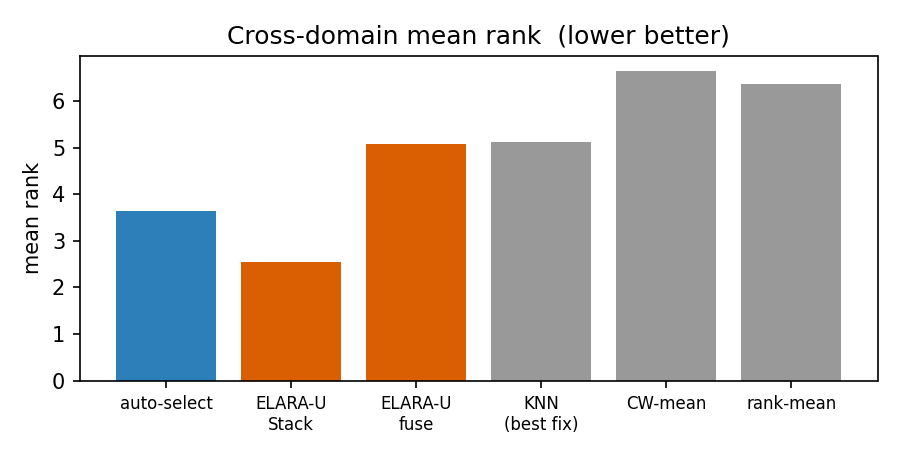
\includegraphics[width=0.95\linewidth]{elara_u_rank.png}
\caption{Cross-domain mean rank over $123$ tasks (lower better). ELARA-U Stack achieves the best average rank on the clean benchmark. (Illustrative; authoritative values in Table~\ref{tab:main}.)}\label{fig:rank}\end{figure}

\begin{figure}[H]\centering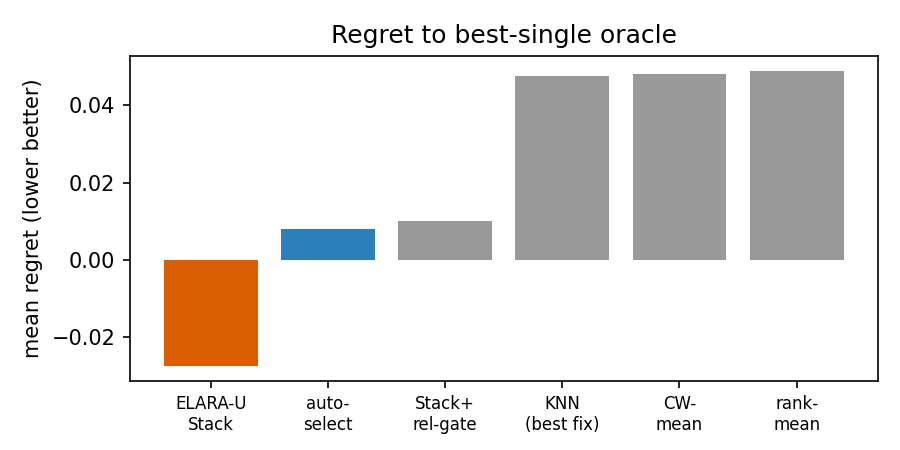
\includegraphics[width=0.95\linewidth]{elara_u_regret.png}
\caption{Mean regret to the per-task oracle. ELARA-U Stack has the lowest regret in the current stress archive.}\label{fig:regret}\end{figure}

\begin{figure}[H]\centering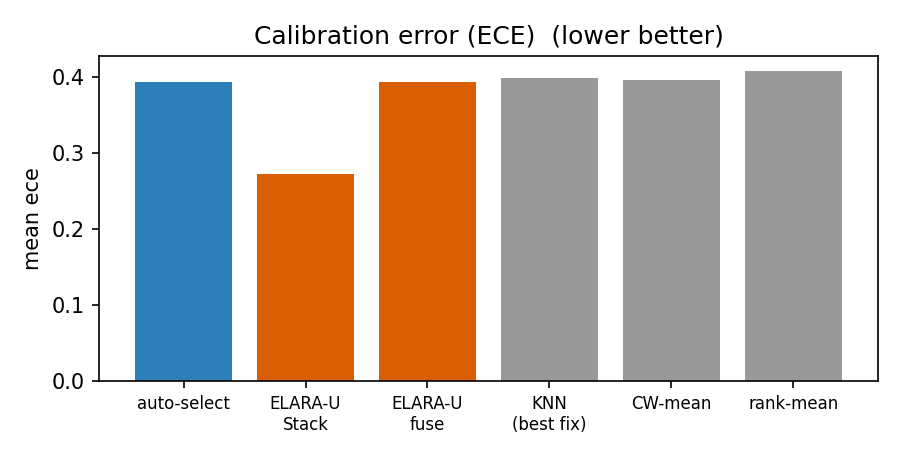
\includegraphics[width=0.95\linewidth]{elara_u_calib.png}
\caption{Calibration error (ECE, lower better). ELARA-U Stack has the best raw ECE; fitted Brier/NLL in Table~\ref{tab:calib}.}\label{fig:calib}\end{figure}

\begin{figure}[H]\centering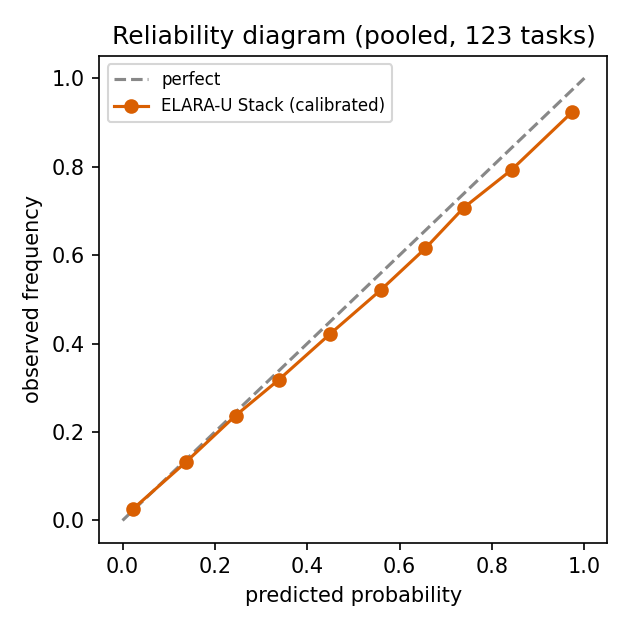
\includegraphics[width=0.55\linewidth]{elara_u_reliability.png}
\caption{Reliability diagram for the isotonic-calibrated ELARA-U Stack, pooled over 123 tasks (calibrator fit on validation only). Points near the diagonal indicate good calibration; Brier/NLL in Table~\ref{tab:calib}.}\label{fig:reliability}\end{figure}

\begin{figure}[H]\centering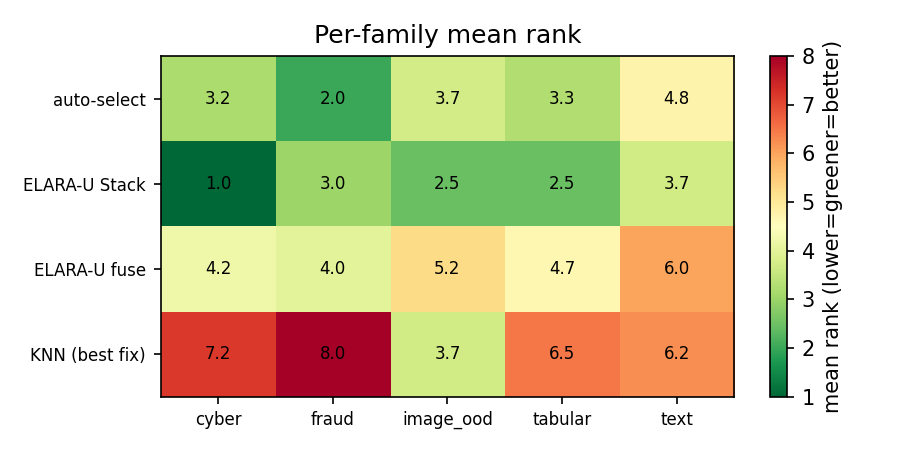
\includegraphics[width=0.95\linewidth]{elara_u_family_heatmap.png}
\caption{Per-family mean rank (greener = better).}\label{fig:heatmap}\end{figure}

\begin{figure}[H]\centering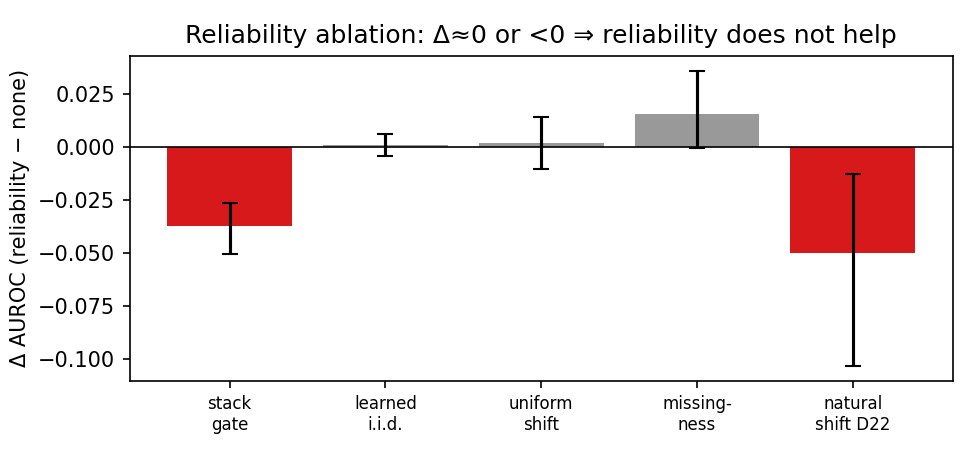
\includegraphics[width=0.95\linewidth]{elara_u_ablation.png}
\caption{Component ablation summary. The stack gain comes from rank-normalized per-task stacking; reliability/drift feature ablations are decisive and \emph{negative} (Table~\ref{tab:ablation}). (Illustrative; authoritative values in Table~\ref{tab:ablation}.)}\label{fig:ablation}\end{figure}

\begin{figure}[H]\centering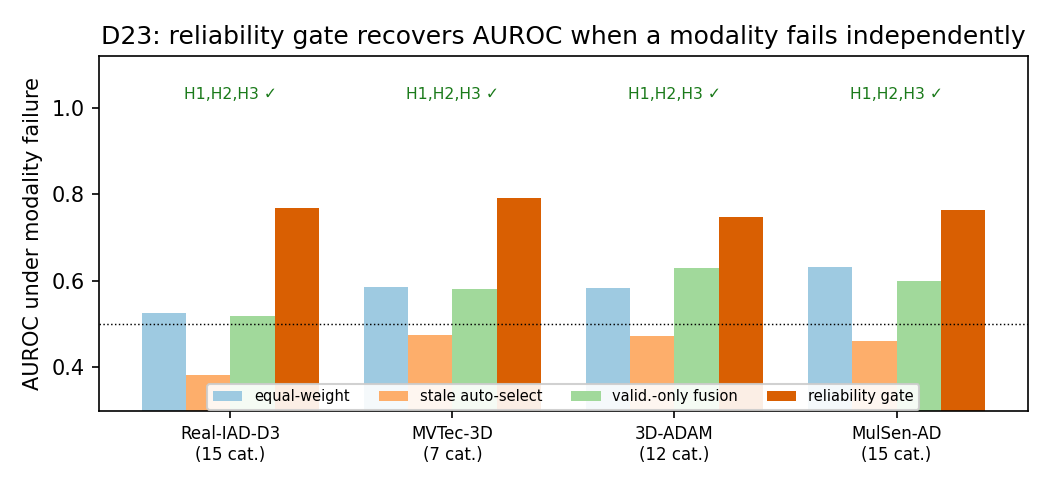
\includegraphics[width=0.98\linewidth]{elara_u_d23_multidataset.png}
\caption{Multimodal independent-modality-failure regime (D23) on \emph{four} real
datasets under the canonical noise protocol. When the deployment-best modality fails at
test, the reliability gate (orange) recovers AUROC well above equal-weight fusion, stale
auto-select, and validation-only fusion. ``H1,H2,H3 \checkmark'' marks datasets where all
three pre-registered hypotheses pass --- all four do. Authoritative deltas and CIs in
Table~\ref{tab:d23}.}\label{fig:d23}\end{figure}

\begin{figure}[H]\centering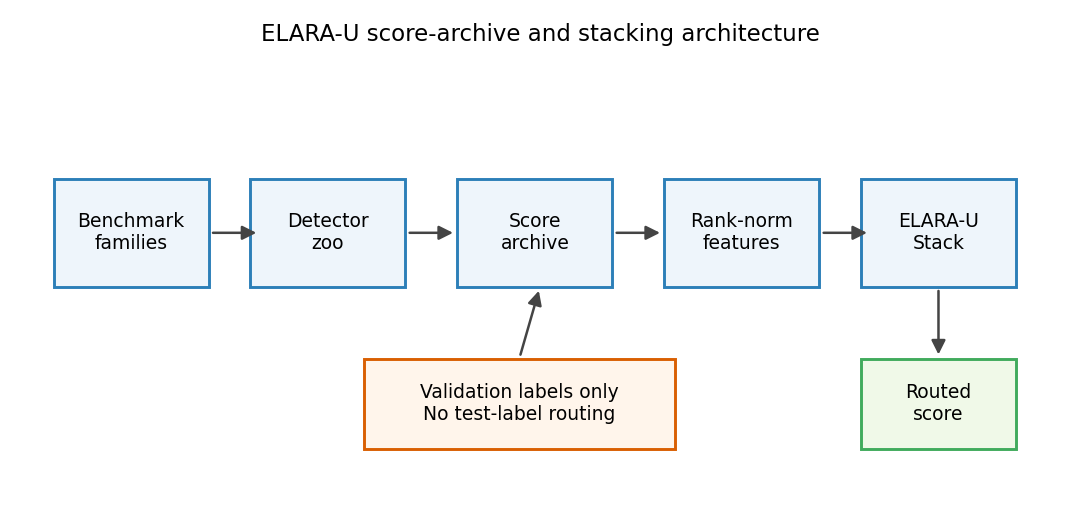
\includegraphics[width=0.95\linewidth]{elara_u_architecture.png}
\caption{ELARA-U architecture: benchmark families feed a detector zoo and score archive; validation-only labels and unlabeled deployment scores drive the router.}\label{fig:arch}\end{figure}

\begin{figure}[H]\centering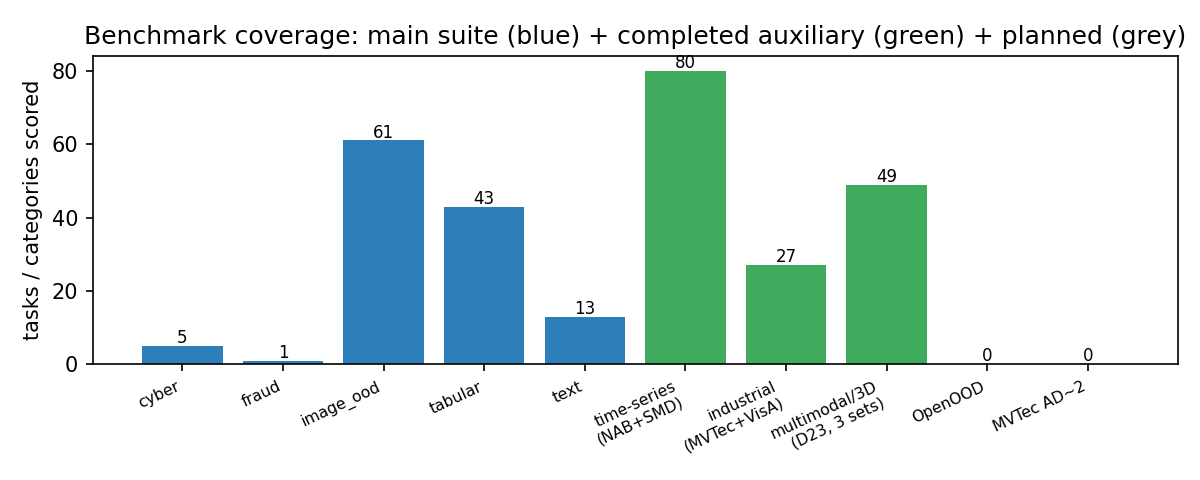
\includegraphics[width=0.95\linewidth]{elara_u_coverage.png}
\caption{Benchmark coverage map. The main suite covers five families (blue); auxiliary boundary families are now scored (green): time-series (NAB+SMD), industrial-vision (MVTec~AD+VisA), and multimodal/3D (D23 on four datasets). OpenOOD and MVTec~AD~2 remain planned (grey).}\label{fig:coverage}\end{figure}

\begin{figure}[H]\centering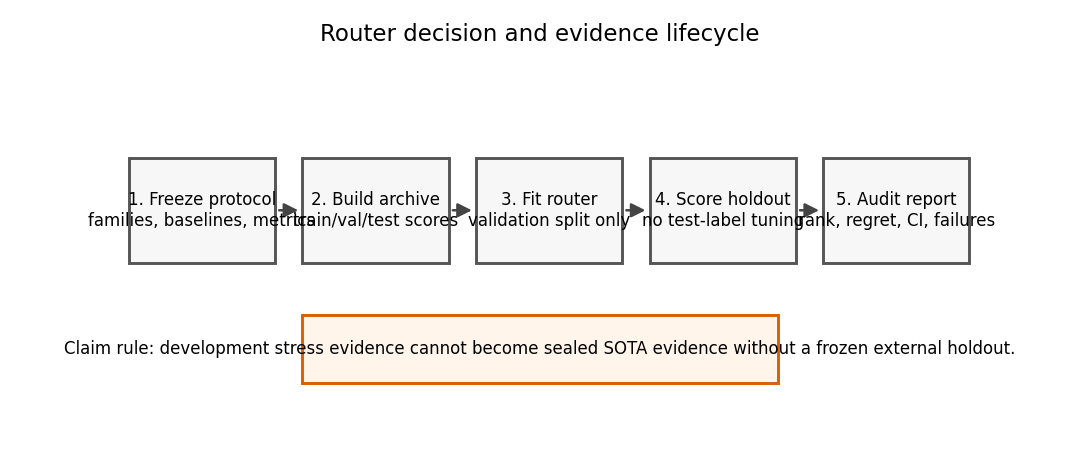
\includegraphics[width=0.95\linewidth]{elara_u_lifecycle.png}
\caption{Router decision lifecycle and evidence boundary. Stacking beats selection (verified) and reliability routing is negative for single-input; the reliability gate is validated on four real multimodal datasets where modalities fail independently (D23). Sealed external evidence still bounds any universal-SOTA claim.}\label{fig:lifecycle}\end{figure}


\section{Scope, Limitations, and Honest Boundaries}
This is a pilot. We do not claim universal superiority or per-dataset SOTA; the
strict clean-transfer gate of the source system remains closed by proof (T9) and
is not relitigated here. We note that while \systemu{} significantly improves the mean rank on cyber, tabular, and image-OOD families, the rank-gain bootstrap interval on text tasks is directionally positive but does not exclude zero, and fraud is underpowered with $n=1$ in the leave-family-out cross-validation. Furthermore, beyond synthetic degradation we ran a sealed natural temporal-shift benchmark (D22, Results): there too plain stacking wins and the drift-aware router is worse (directionally; the $n{=}7$ negative does not survive Holm correction, while the 123-task stack-gate negative does), so the reliability/drift machinery does not help even under natural shift; native OOD and industrial sensor-drift families remain future work. Calibration is now reported with fitted Brier and NLL (Table~\ref{tab:calib}, reliability diagram Fig.~\ref{fig:reliability}); larger sealed natural-shift suites remain future work.

\section{Reproducibility}
Router and evaluation: \texttt{src/scripts/elara\_u/gate\_u\_seed\_eval.py};
contract: \texttt{research\_lock/GATE\_U\_CROSS\_DOMAIN\_PROTOCOL\_v1.yaml};
results: \texttt{experiments/elara\_u/}. No test labels enter router fitting
(audited in Algorithm~\ref{alg:router-train}).

\clearpage
\appendix
\section{Theoretical Proofs and Extensions}
\label{sec:theory_appendix}

\subsection{Supporting Propositions and Lemmas}

\begin{proposition}[Rank-Normalized Stacking Invariance]
\label{prop:rank_invariance}
Let detector $m$ produce scores $s_m(x)$, and let $h_m:\mathbb{R}\to\mathbb{R}$ be any strictly increasing transformation. Define the normalized rank feature
\[
r_m(x)=\frac{1}{n}\sum_{i=1}^n \mathbf{1}\{s_m(x_i)\leq s_m(x)\}.
\]
Then replacing $s_m(x)$ with $h_m(s_m(x))$ leaves $r_m(x)$ unchanged for every sample $x$, up to tie-handling. Therefore, any ELARA stacker using only detector-wise rank-normalized features is invariant to monotone score rescaling, calibration drift, or sensor-scale drift.
\end{proposition}
\begin{proof}
For any two samples $(x_i,x_j)$,
\[
s_m(x_i)\leq s_m(x_j)
\]
if and only if
\[
h_m(s_m(x_i))\leq h_m(s_m(x_j)),
\]
because $h_m$ is strictly increasing. Therefore, the ordering of all samples under detector $m$ is unchanged. Since $r_m(x)$ depends only on the ordering of scores and not on their numerical scale, $r_m(x)$ is unchanged. Any downstream stacker that receives only $r_m(x)$ is therefore invariant to such monotone transformations.
\end{proof}

\medskip
\noindent\textbf{Interpretation.}
This proposition justifies the rank-normalized stacking design. It protects the router from meaningless score-scale changes while preserving anomaly ranking information.

\begin{proposition}[Degenerate-Channel Guard for Saturation]
\label{prop:degenerate_guard}
Let a fused anomaly score be
\[
g(x)=\sum_{m=1}^M w_m s_m(x),
\qquad w_m\geq 0,\qquad \sum_m w_m=1.
\]
If detector $k$ is saturated on validation data so that
\[
\mathrm{Var}_V(s_k)\leq \epsilon,
\]
then replacing $w_k$ by $0$ and renormalizing the remaining weights changes pairwise score differences by at most $O(\sqrt{\epsilon})$. In the limit $\epsilon\to 0$, the saturated detector contributes no ranking information, and removing it cannot remove meaningful rank signal.
\end{proposition}
\begin{proof}
For any two samples $(x_i,x_j)$,
\[
|s_k(x_i)-s_k(x_j)|
\leq
O(\sqrt{\epsilon})
\]
by the bounded-variance assumption. The contribution of detector $k$ to the fused pairwise difference is
\[
w_k(s_k(x_i)-s_k(x_j)),
\]
which is also $O(\sqrt{\epsilon})$. Therefore, as $\epsilon\to 0$, detector $k$'s contribution to every pairwise ranking comparison vanishes. Removing $k$ and renormalizing the remaining non-degenerate detectors does not remove meaningful rank information from the fused score.
\end{proof}

\medskip
\noindent\textbf{Interpretation.}
This supports the degenerate-channel guard for saturated detectors. A detector that produces nearly constant scores should not influence routing or fusion.

\begin{proposition}[Inverted Detector Harm Under Positive Fusion]
\label{prop:inverted_harm}
Assume the clean fused margin between an anomalous and normal sample is
\[
D_0=g_0(X^+)-g_0(X^-),
\]
with $\mathbb{E}[D_0]>0$. Suppose an inverted detector $k$ has margin
\[
D_k=s_k(X^+)-s_k(X^-)
\]
with $\mathbb{E}[D_k]<0$. For a positive fusion weight $w>0$, the fused margin
\[
D_w=(1-w)D_0+wD_k
\]
satisfies
\[
\mathbb{E}[D_w]
=
(1-w)\mathbb{E}[D_0]+w\mathbb{E}[D_k]
<
\mathbb{E}[D_0].
\]
Under a Gaussian equal-variance margin model, AUROC is monotone increasing in the standardized margin mean. Therefore, assigning positive weight to an inverted detector decreases AUROC relative to zeroing it.
\end{proposition}
\begin{proof}
The expectation follows from linearity:
\[
\mathbb{E}[D_w]
=
(1-w)\mathbb{E}[D_0]+w\mathbb{E}[D_k].
\]
Since $\mathbb{E}[D_k]<0<\mathbb{E}[D_0]$, we have $\mathbb{E}[D_w]<\mathbb{E}[D_0]$.
Under the Gaussian equal-variance margin model,
\[
D_w\sim \mathcal{N}(\mu_w,\sigma^2),
\]
and
\[
\mathrm{AUROC}(g_w)=\Pr[D_w>0]=\Phi\left(\frac{\mu_w}{\sigma}\right).
\]
Because $\Phi$ is strictly increasing and $\mu_w<\mu_0$, positive weight on the inverted detector decreases AUROC.
\end{proof}

\medskip
\noindent\textbf{Interpretation.}
This proposition supports validation-based inversion guards. If a detector is reliably below chance, positive-weight fusion can harm ranking.

\begin{proposition}[Meta-Router Generalization Requires Enough Tasks]
\label{prop:generalization_tasks}
Let $\mathcal{H}$ be a finite class of meta-routers, and let the task-level loss $\ell(h,\tau)\in[0,1]$ denote normalized rank regret or negative-transfer loss. Given $T$ independent meta-training tasks, with probability at least $1-\delta$, every router $h\in\mathcal{H}$ satisfies
\[
L(h)
\leq
\widehat{L}_T(h)
+
\sqrt{\frac{\log|\mathcal{H}|+\log(1/\delta)}{2T}},
\]
where $L(h)=\mathbb{E}_\tau[\ell(h,\tau)]$ is the expected held-out task loss and $\widehat{L}_T(h)=\frac{1}{T}\sum_{t=1}^T\ell(h,\tau_t)$ is the empirical meta-training loss.
\end{proposition}
\begin{proof}
For any fixed $h$, Hoeffding's inequality gives
\[
\Pr\left(
L(h)-\widehat{L}_T(h)>\epsilon
\right)
\leq
\exp(-2T\epsilon^2).
\]
Applying a union bound over all $h\in\mathcal{H}$,
\[
\Pr\left(
\exists h\in\mathcal{H}: L(h)-\widehat{L}_T(h)>\epsilon
\right)
\leq
|\mathcal{H}|\exp(-2T\epsilon^2).
\]
Set the right-hand side equal to $\delta$:
\[
|\mathcal{H}|\exp(-2T\epsilon^2)=\delta.
\]
Solving for $\epsilon$ gives
\[
\epsilon=
\sqrt{\frac{\log|\mathcal{H}|+\log(1/\delta)}{2T}}.
\]
Thus, with probability at least $1-\delta$, the stated bound holds for every $h\in\mathcal{H}$.
\end{proof}

\medskip
\noindent\textbf{Interpretation.}
This explains why ELARA needs many tasks and leave-family-out evaluation. A high-capacity router trained on too few tasks can overfit meta-level structure and fail to generalize.

\subsection{Old ELARA/RGA Source-System Theory Stack}

Below are the foundation certificates and bounds inherited from the ELARA/RGA source-system framework.

\begin{certificate}[Switching Certificate]
\label{cert:switch}
Let $\Delta_{\mathrm{fired}} = A(\mathrm{route}) - A(\mathrm{default})$ be the routed-minus-default performance on the subset of inputs where the router fires. The router may replace the default \emph{only if} the one-sided level-$\alpha$ lower confidence bound satisfies $\mathrm{LCB}_{1-\alpha}(\Delta_{\mathrm{fired}}) > 0$. Under this rule the expected switch is non-negative at level $\alpha$: routing is admitted only with certified fired-set benefit, never on a point estimate.
\end{certificate}

\begin{diagnostic}[Mean-Reliability Dilution]
\label{diag:dilution}
Let per-expert reliabilities be $r_1,\dots,r_M$ with mean $\bar r=\tfrac1M\sum_m r_m$ and gate threshold $\tau$. There exist configurations with $\bar r > \tau$ while a minority expert collapses ($r_k\to 0$): mean-gating does not fire and the collapsed expert is still trusted. The miss probability is $P(\mathrm{miss})=\Phi\!\big((\bar\mu-\tau)/\bar\sigma\big)$; detecting minority collapse requires per-expert / min-gating, not the mean (Theorem~T3).
\end{diagnostic}

\begin{slack}[Router Generalisation Slack]
\label{prop:slack}
Let the router class have complexity $C$ (e.g.\ VC dimension or Rademacher complexity) and let the meta-training set contain $T$ tasks. The gap between meta-training and held-out expected rank-gain is bounded by $O\!\big(\sqrt{C/T}\big)$ with high probability. Hence the evidential strength of a routing claim requires $T \gtrsim C$: a high-capacity router over few tasks yields weak evidence even at a positive point estimate. This motivates a large, heterogeneous benchmark suite (the Gate U minimum-viable families) before any claim.
\end{slack}





\end{document}
